\documentclass[a4paper,12pt]{article}
\usepackage[utf8]{inputenc}
\usepackage{polski}
\usepackage{graphicx}
\usepackage{amsmath}
\usepackage{amssymb}
\usepackage{hyperref}

\title{Sprawozdanie z laboratorium Hurtownie Danych}
\author{Mikołaj Kubś, 272662}
\date{\today}

\begin{document}

\maketitle

\section{Zadanie 1}
Analiza konceptualnego modelu danych "Usługi", który jest niekompletny,
ale klasy i relacje między nimi reprezentują rozpatrywany wycinek rzeczywistości. 

\begin{figure}[h!]
\centering
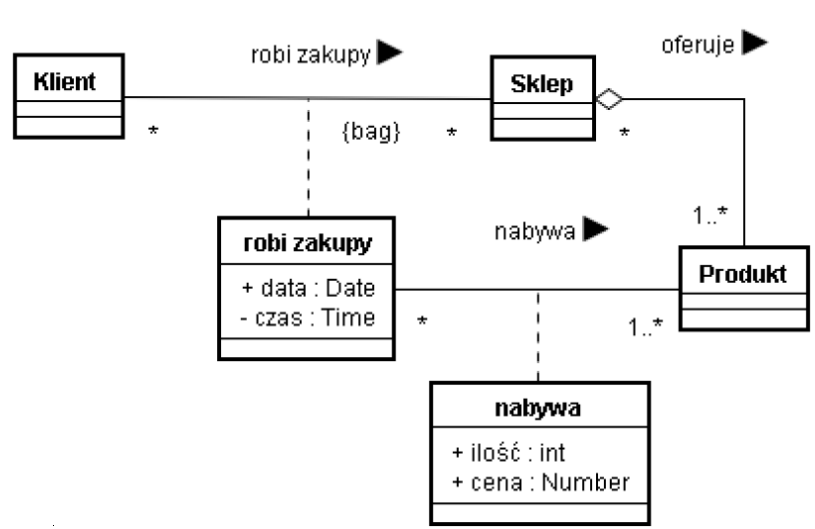
\includegraphics[width=0.8\textwidth]{images/image1.png}
\caption{Konceptualny model danych "Usługi"}
\label{fig:uslugi}
\end{figure}

Reguły i ograniczenia dziedzinowe:
\begin{itemize}
    \item Reg/01 - Klient może wielokrotnie robić zakupy w tym samym sklepie
    \item Reg/02 - W sklepie może robić zakupy dowolny klient
    \item Reg/03 - Każdy zakup realizowany jest przez klienta w sklepie w określonym dniu i godzinie
    \item Reg/04 - Sklep musi oferować co najmniej jeden produkt
    \item Reg/05 - \ldots
\end{itemize}

\subsection{Weryfikacja i poprawa modelu danych}

Ponieważ reguły są niekompletne i nie w pełni poprawne, zdecydowałem się wprowadzić szereg zmian. 

Uznałem, że reguła "Reg/04 - Sklep musi oferować co najmniej jeden produkt" wprowadza niepotrzebną komplikację. Na przykład, według tej zasady, gdy sklep sprzedałby cały swój inwentarz, nie mógłby dalej istnieć w bazie danych.

Brakuje aktualnie informacji, jaka jest liczba dostępnego produktu w danym sklepie. Można wyciągnąć tą daną do nowej tabeli asocjacyjnej, do której można by dodatkowo dodać cenę produktu dla konkretnego sklepu, co zwiększa elastyczność na przyszłość i jest szeroko stosowaną praktyką. Tak więc sklep może mieć oferować wiele produktów, każdy z własną cenę i ilością. Ponieważ tabela asocjacyjna "oferuje" ma cenę, można by usunąć cenę z tabeli asocjacyjnej "nabywa". Uznałem jednak, że ją zostawię, ponieważ cena oferty może się zmienić po zakupie produktu przez klienta.

Można dodać parę atrybutów do niektórych encji. Do klienta dodam imię i nazwisko.

Warto również dodać ograniczenia wobec atrybutów encji. Warto również dodać reguły klaryfikujące, że:

\begin{enumerate}
    \item klient może robić zakupy w różnych sklepach
    \item ten sam produkt może być oferowany w wielu sklepach
    \item klient robiący zakupy musi zakupić przynajmniej 1 produkt
\end{enumerate}

Reguły te są logiczne i wynikają z podanego wcześniej konceptualnego modelu danych.

Dodatkowo zmieniłem typ atrybutów dotyczących kosztu na "decimal", a także zmieniłem atrybut "data" w "robi zakupy" na prywatny.

\subsection{Finalna postać reguł, ograniczeń i diagramu klas UML}

Finalna postać reguł i ograniczeń:

\begin{itemize}
    \item Reg/01 - Klient może wielokrotnie robić zakupy w tym samym sklepie
    \item Reg/02 - W sklepie może robić zakupy dowolny klient
    \item Reg/03 - Każdy zakup realizowany jest przez klienta w sklepie w określonym dniu i godzinie
    \item Reg/04 - Każdy sklep ustala własną cenę oraz ilość oferowanego produktu 
    \item Reg/05 - Klient nabywając produkt w danym sklepie kupuje go za cenę oferowaną w sklepie, która zostaje zapamiętana
    \item Reg/06 - Sklep może zmienić cenę oferowanego produktu, co wpływa tylko na przyszłe zakupy
    \item Reg/07 - Klient może robić zakupy w różnych sklepach
    \item Reg/08 - Ten sam produkt może być oferowany w wielu sklepach
    \item Reg/09 - Klient robiąc zakupy musi nabyć co najmniej 1 produkt
    \item Reg/10 - Imię klienta nie może być puste
    \item Reg/11 - Nazwisko klienta nie może być puste
    \item Reg/12 - Cena oferowanego produktu nie może być mniejsza od zera
    \item Reg/13 - Ilość nabytego produktu musi być większa od zera
    \item Reg/14 - Cena nabytego produktu nie może być mniejsza od zera
\end{itemize}

\begin{figure}[h!]
\centering
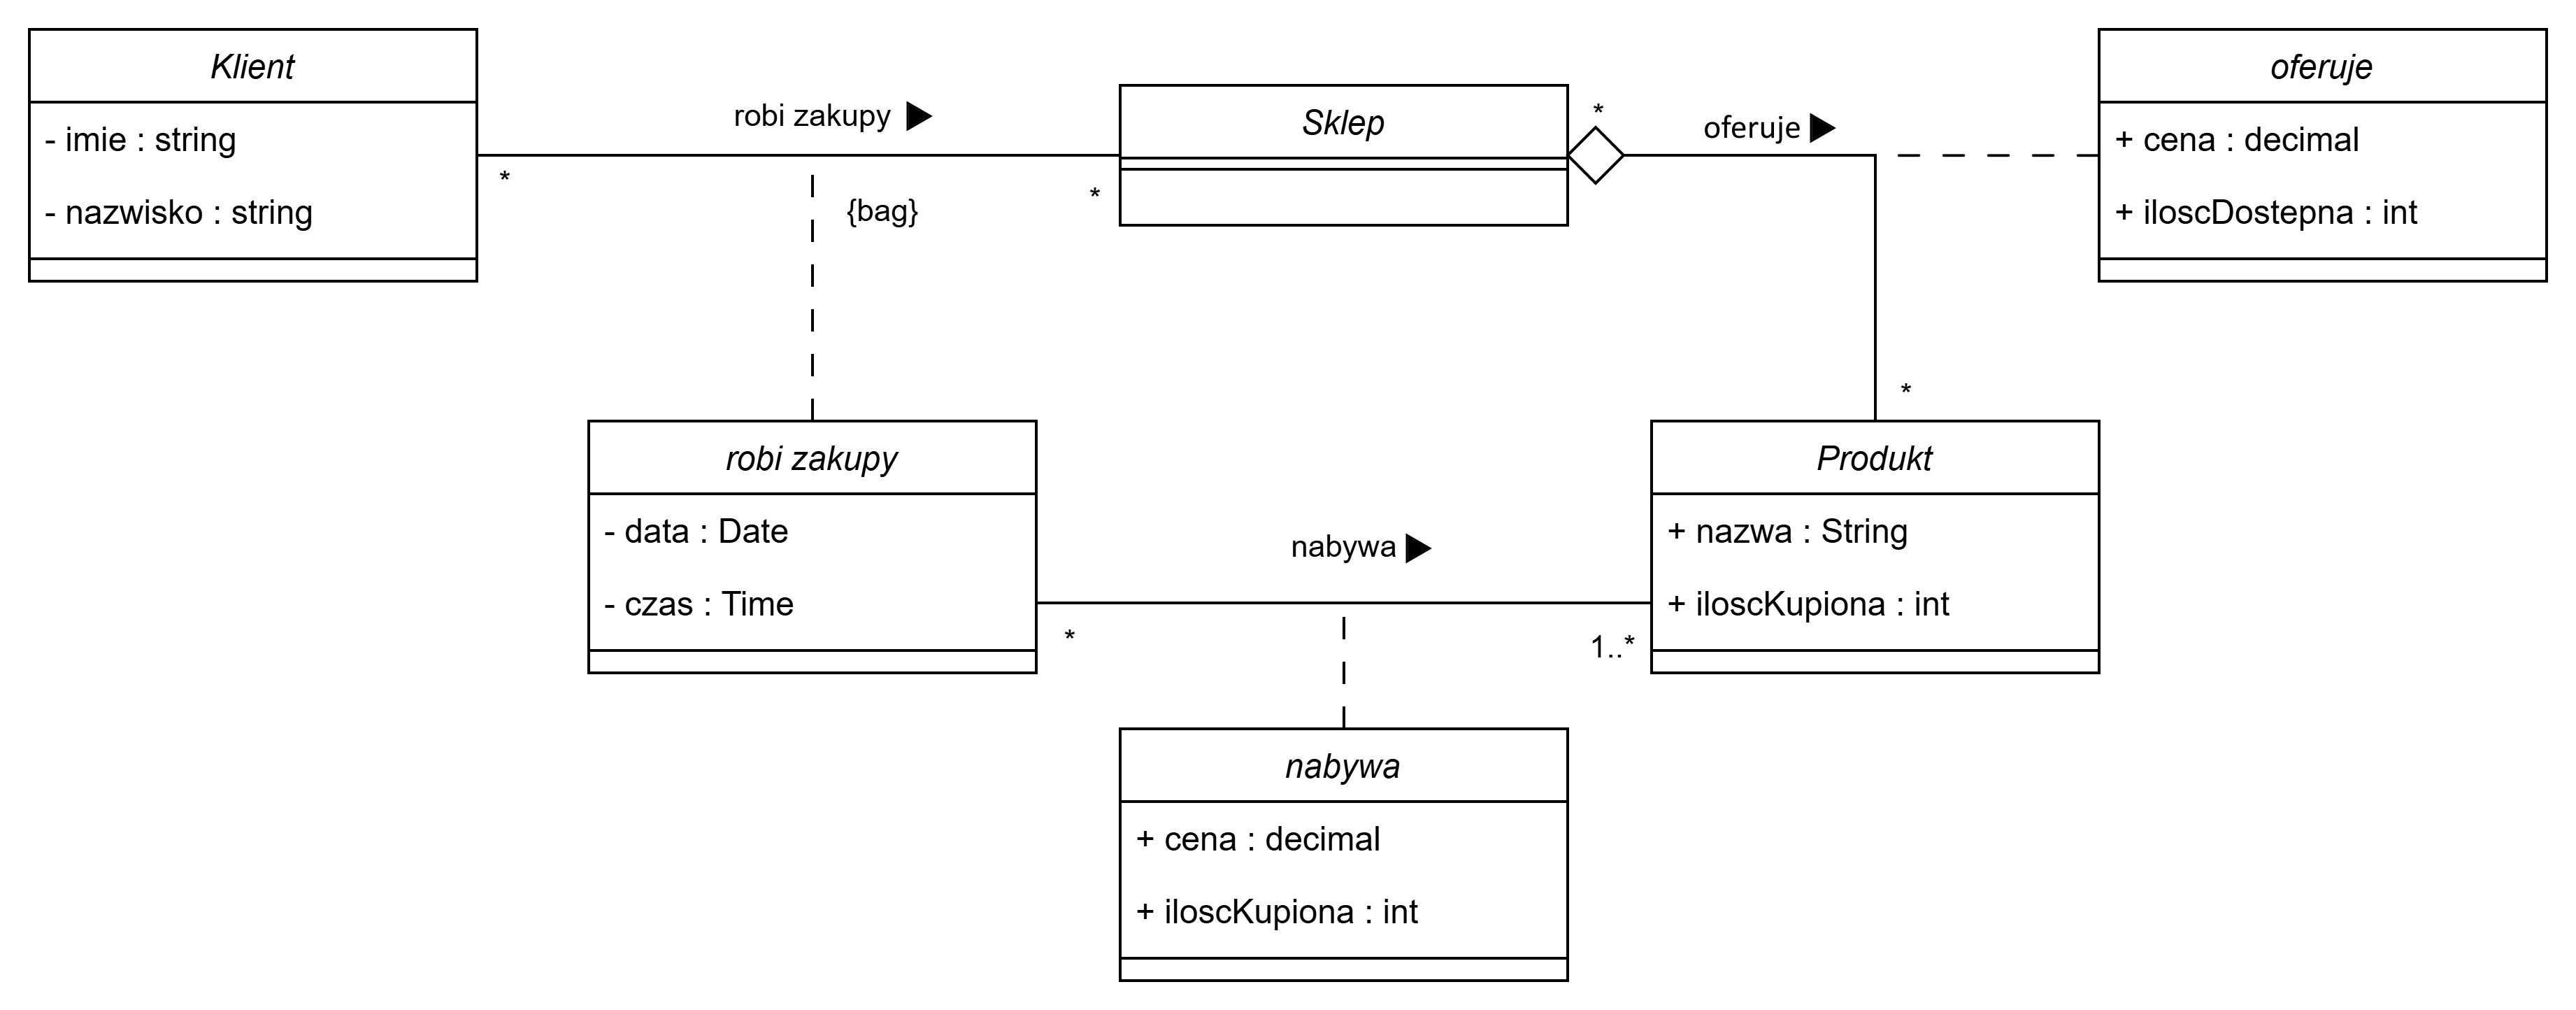
\includegraphics[width=0.8\textwidth]{images/improved.png}
\caption{Finalny model danych "Usługi"}
\label{fig:final_model}
\end{figure}

\subsection{Skrypt DDL SQL}

\section{Zadanie 2}
Tutaj znajduje się cel laboratorium.

\begin{thebibliography}{9}
\bibitem{przyklad}
Autor, \textit{Tytuł}, Wydawnictwo, Rok.
\end{thebibliography}

\end{document}